\section{Implementation}
On the background of the chosen design from the design section, a prototype will be built and later used for testing.
Throughout this section, there will be a presentation and discussion of how this prototype has been implemented. 
The implementation consists of two parts: first a software part, where the programming of the application will be described, and second, a description of the physical artefacts that will be used for testing.

\subsection{Physical artefacts}
As explained in the chosen design, the idea with the physical artefact used as a part of the game controller, is that the user should be able to fully customize it him-/herself. 
In order to create a prototype usable for testing, a simple wheel-like controller has been created used to control the acceleration, braking/reversing, camera view and steering of the car. 
Additionally, to shift gear up and down, a yellow sponge was used and managed with the right hand. 
In figure \ref{fig:imp1} a picture of both the sponge and the wheel-like controller is shown. 
The sponge is used as the yellow colour is fairly easy to distinguish from other colours. 
The wheel controller in the right side of the figure is made of a piece of cardboard with an attached A4-sized piece of paper, on which is printed three colours. 
This wheel has the two main colours, red and blue, which are used as fixation points to determine the right and the left side of wheel. 
These two creations, the sponge and the wheel, are examples of how a user could choose to design his/her own controller.
\bigskip

\begin{figure}[!htbp]
\centering
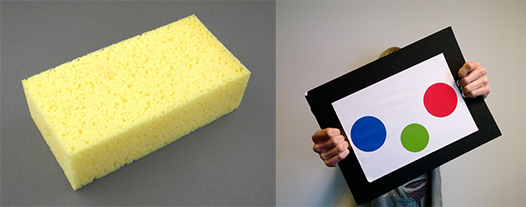
\includegraphics[width=4in]{Imp1}
\caption{The physical part of the racing game controller. (left) A sponge is used to change gear and (right) a wheel-like controller is used to steer, accelerate/decelerate the car and change camera view.} 
\label{fig:imp1}
\end{figure}

The way the wheel controller is used, is by rotating it, like a typical vehicle wheel, in order to turn the car in the game. 
Also, the wheel can be moved towards and away from the camera to accelerate and decelerate accordingly, while moving the wheel to either the left or the right will activate an extra function in the game, which here has been chosen to be changing the camera view. 
The sponge, however, is used to shift up and down in gear by raising or lowering it with the right hand accordingly. 
This means, that in order to change gear, the user will have to release the wheel with the right hand to raise/lower the sponge in front of the webcam, which again is an example of how a user can freely choose how he/she wants to manage those three required fixation points.

\subsection{Development of the software application}
The main part of this prototype consists of a piece of software developed for registering input from the user and deliver this information to a racing game, which will give the user the ability to control a car in a game. 
The software that will be described in this chapter is based on the programming language C++. 
As the idea of registering input from the user is based on visual computing, the open source C++ toolkit “openFrameworks” has been used, as this toolkit works very well with visual computing.
To describe the software developed for this prototype, first a walkthrough of the flow of the application will be presented followed by a description of specific parts of the code.

\subsubsection{Flow of the application}
To be able to use the controller the user has to start up the software on a computer with a webcam connected to it. 
In figure \ref{fig:imp2}, a flowchart of what happens when the user does certain things is presented. 
Starting from the top left of the figure, a dot represents the user starting the program, which immediately leads the program to the main menu.
\bigskip

\begin{figure}[!htbp]
\centering
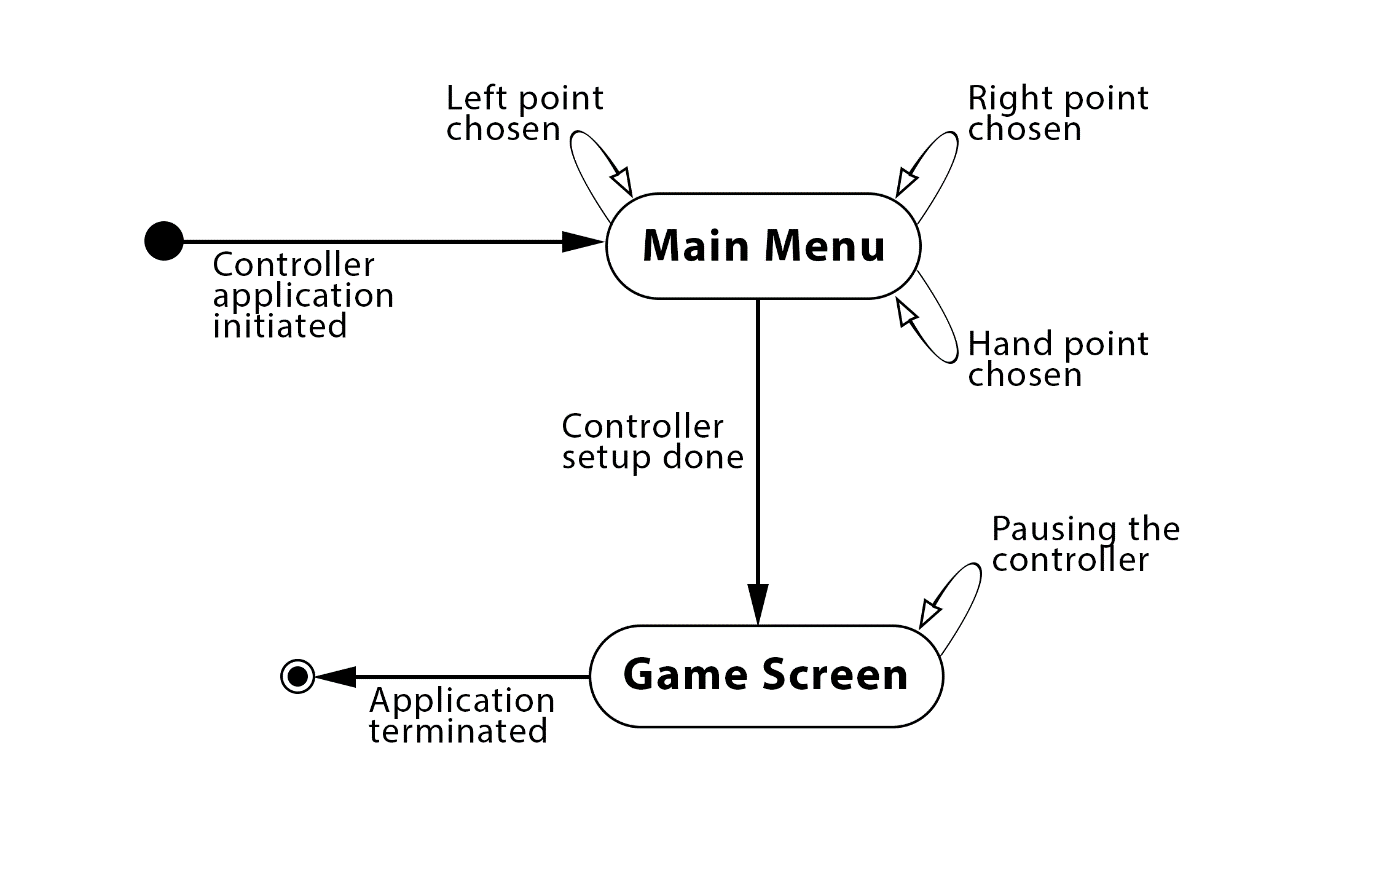
\includegraphics[width=4in]{Imp2}
\caption{State chart.} 
\label{fig:imp2}
\end{figure}

In the main menu, the user is asked to give some information about which colours, in the image captured by the webcam, are used as the left and right point of the wheel-part of the controller. 
These two colours are chosen by marking the area in the image, in which each of the colours are represented. 
In figure \ref{fig:imp3} an example of choosing the colours can be seen. 
First, the left point (the red colour on the controller) has been chosen, by clicking on the little box to the left of the text saying “Add left point”.
Hereafter, the user has to click and drag on the image to the left in the figure around a part of the red mark on the controller. 
The program then finds all the red-coloured pixels in the left image and represents them in the right image as pure red pixels. 
After choosing the left point, the right point can be chosen, which is the ongoing action in the figure. 
The last point, “hand point”, is the colour that should represent the gear-shifting controller, described as the yellow sponge earlier.
\bigskip

\begin{figure}[!htbp]
\centering
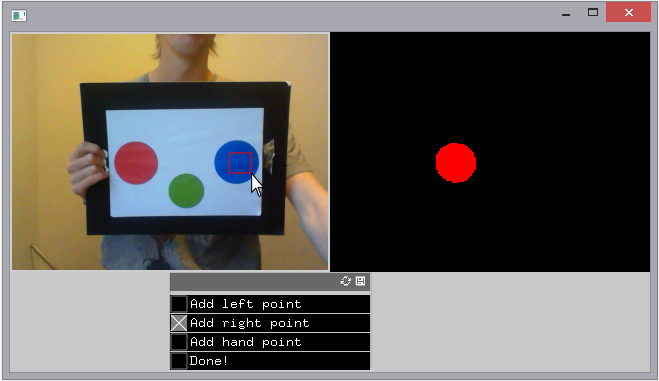
\includegraphics[width=4in]{Imp3}
\caption{Window showing selection of color tracking.} 
\label{fig:imp3}
\end{figure}

Back in the flowchart in figure \ref{fig:imp2}, the arrows going out and back into the main menu, illustrates that, when the user selects a colour to use as one of the points, it is registered, but the main menu keeps open. 
When the user clicks “Done!” (see figure \ref{fig:imp3}), the setup of the controller points is finished, which leads the program to the game screen. 
The game screen takes care of registering what the user does in order to tell the car in the game how to behave. 
An example of how the game screen looks when the program is running can be found in figure \ref{fig:imp4}. 
Here, each of the points are shown as the red, green and blue circles on the left image, while the yellow circle is the centre point between the right and left point of the wheel controller. When the yellow circle is moved either to the left or the right of the magenta box, the camera view in the game will be changed. 
A more thoroughly description of the game screen, including how the other game actions are activated, will be presented in the following chapter (\ref{sec:codedesc} Code description).
\bigskip

\begin{figure}[!htbp]
\centering
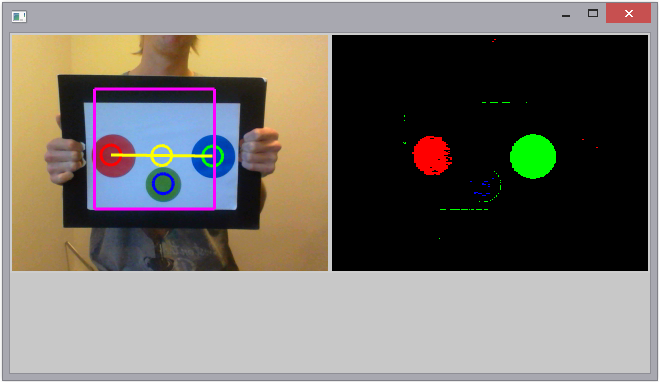
\includegraphics[width=4in]{Imp4}
\caption{Window showing active tracking.} 
\label{fig:imp4}
\end{figure}

When the game screen is shown, it is possible to put it on pause, if the user for some reason would have to temporarily turn off the controller. 
In the flowchart on figure \ref{fig:imp2}, this is illustrated as the arrow going out from and back into the game screen. 
When the user finally wants to turn off the controller, the application can be terminated by either pressing the escape button (esc) or clicking the X in the top right of the window, which in the flowchart is represented as the arrow pointing to the dot surrounded by a circle. 
At this point, the application will no long be running, which stops the flow of the program.

\subsubsection{Code description} \label{sec:codedesc}
In this chapter, important and/or interesting parts of the code behind the software will be presented and described in order to show how the actions performed by the user will result in some actions on the screen. 
Furthermore, the use of image/video processing and analysis will be explained as to how this piece of software obtains and utilizes input from the user through images/a video stream captured by the webcam.

\subsubsection*{Main Menu}
The mainMenu.cpp file takes care of letting the user select three areas of interest on the screen, and then shows the user what is being detected. 
The user can also reselect areas, if the detection doesn’t seem right to them. 
When the user has selected three areas and presses the “Done!” button, the gameScreen.cpp file will be run.
\bigskip

\pagebreak[4]
\begin{lstlisting}[caption=mousePressed function, label=lst:lst1]
void mainMenu::mousePressed(int x, int y, int button)
{
    //Initiates the rectangle when the user presses a mouse button.
    selectStart.x = x;
    selectStart.y = y;
    selectEnd.x = x;
    selectEnd.y = y;
    selectionRect.set(selectStart, selectEnd);
    drawRect = true; //Starts drawing the rectangle visually
}

\end{lstlisting}

The function in snippet \ref{lst:lst1} is activated every time the user presses a button on the mouse. 
When that happens, the x and y value for selectStart and selectEnd are set to the current position of the mouse. 
The function is the first step in drawing a rectangle on the screen and analyzing the selected pixels. 
selectStart needs to be given values, as this is the first corner of the rectangle. 
selectEnd needs values from the beginning, in case the user only clicks on the image, thereby selecting only one pixel.
selectionRect.set defines how the rectangle should be drawn on the screen; in this case a rectangle should be made based on the two defined points (selectStart and selectEnd).
Lastly, this function sets drawRect to true, so another function knows that it should draw the rectangle on the screen.
\bigskip

\begin{lstlisting}[caption=mouseDragged function, label=lst:lst2]
void mainMenu::mouseDragged(int x, int y, int button){
    //Updating the rectangle values when the user is dragging the mouse across the screen.
    selectEnd.x = x;
    selectEnd.y = y;
    selectionRect.set(selectStart, selectEnd);
}

\end{lstlisting}

Snippet \ref{lst:lst2} takes care of what should happen when the user drags the mouse over the screen, while holding down a mouse button. 
Since selectStart needs to be stationary, and drawRect is already true, only selectEnd is changed to the current position of the mouse, updating the rectangle when the user drags the mouse. 
selectionRect is also updated to give the user visual feedback.
\bigskip

\pagebreak[4]
\begin{lstlisting}[caption=mouseReleased function, label=lst:lst3]
void mainMenu::mouseReleased(int x, int y, int button){
    if(leftPointBtn){
        leftPointBtn = false; //Sets the toggle button back to false when a selection has been made.
        saveVals(selectStart, selectEnd, leftVals); //Saves the colors in the rectangle for detection.
        leftIsActive = true; //This color is now being detected as the left point.
    }
    if(rightPointBtn){...}
    if(handPointBtn){...}
    drawRect = false; //Stops drawing the rectangle
}
\end{lstlisting}

Snippet \ref{lst:lst3} activates whenever the user release a mouse button.
The 3 if-statements check what selection is being made (chosen by the user pressing one of the three buttons on the screen). 
Only the leftPointBtn if-statement will be explained, since the other if-statements does exactly the same, except the values being changed are called “right” or “hand” instead of “left”. 
First, the leftPointBtn (buttons on the screen) is set to false. Then the program runs the “saveVals” function, which finds the colours that should be thresholded, based on the selected pixels. 
These threshold values are saved in the “leftVals” array.
leftIsActive is then set to true, telling the program that some values have been selected for the “left” values.
Lastly, drawRect is set to false, telling the program that the rectangle should no longer be drawn on the screen.
\bigskip

Snippet \ref{lst:lst4} finds the threshold values and inserts them into an array. 
Note that parts of this function have been excluded in this snippet, so only the core remains. 
The function goes through each of the selected pixels, converts each of the pixels from the RGB (red, green, blue) colour space, to HSV (hue, saturation, value). 
The hue values of each pixel are then pushed into an array in the form of a vector. 
It then sorts these values, from lowest to highest, and finds the median hue value of all the pixels in the array, by picking the center one. 
This hue value is then inserted into an array, together with the lowest saturation and lowest value, defined as sLow and vLow, which are constant values. 
sLow and vLow are defined earlier in the function; sLow is set to 0.5 and vLow is set to 0.3.

\pagebreak[4]
\begin{lstlisting}[caption=saveVals function, label=lst:lst4]
void mainMenu::saveVals(ofPoint p1, ofPoint p2, float *arr){
    //Goes through each selected pixel.
    for(int y = y1; y <= y2; y++){
        for(int x = x1; x <= x2; x++){
            //Pushes all hue values of a pixel into an array.
            r = mirrorOut[int(w * y + x)*3+0];
            g = mirrorOut[int(w * y + x)*3+1];
            b = mirrorOut[int(w * y + x)*3+2];
            mainMenu::RGB2HSV(r, g, b, &h, &s, &v); //Converts the current pixel to hsv.
            medianHues.push_back(h); //Pushes the hue value into an array.
        }
    }

    sort(medianHues.begin(), medianHues.end()); //Sorts the array of hue values.
    h = medianHues[int(medianHues.size()/2)]; //Finds the median hue value and saves it.

    //Inserts values into an array. This array is used for thresholding so the program knows what colors to detect.
    arr[0] = h;
    arr[1] = sLow;
    arr[2] = vLow;
}
\end{lstlisting}

\begin{lstlisting}[caption=Thresholding, label=lst:lst5]
threshOut[(x+y*w)*3+0] = 0;
threshOut[(x+y*w)*3+1] = 0;
threshOut[(x+y*w)*3+2] = 0;

if(leftIsActive){ //Thresholds the values for the left point (if selected)
    if(h < leftVals[0] + HUE_THRESH && h > leftVals[0] - HUE_THRESH
        && s > leftVals[1]
        && v > leftVals[2]) //leftVals comes comes from a function that is activated when the user selects something.
    {
        threshOut[(x+y*w)*3+0] = 255;
    }
}
if(rightIsActive){...}
if(handIsActive){...}
\end{lstlisting}

Snippet \ref{lst:lst5} is run through each time the program updates. 
First, the current pixel is set to black. 
This ensures that all pixels that aren’t being thresholded will be black. 
Then, the program checks if leftIsActive is true, and if it is, it will threshold colors based on the values in the leftVals array. 
If the current pixel is inside the threshold range, its colour will be changed to red. 
The same will be done for the two last if-statements, setting the colours to green and blue instead, if the pixel is inside the respective threshold range.


\subsubsection*{Game Screen}
The gameScreen.cpp file takes input from the mainMenu.cpp, so it knows what colors to detect. 
The gameScreen.cpp file detects the selected colours, performs a BLOB analysis on these colours, finds the center of the colours, and sends these center-points to the according classes. 
Then it receives input from these classes and takes care of simulating key presses.
\bigskip

\begin{lstlisting}[caption=Post BLOB analysis, label=lst:lst6]
if(detectedPixelsLeft > 0){
    leftPoint.x /= detectedPixelsLeft;
    leftPoint.y /= detectedPixelsLeft;
    leftCircle = leftPoint;
}
\end{lstlisting}

In snippet \ref{lst:lst6} after doing a BLOB analysis, from the found BLOB the program adds each pixel’s x position to a variable and y position to another variable. 
It also counts how many pixels have been detected. 
This piece of code then finds the centre/average, of those pixels by dividing the added x and y values with the total number of pixels in the BLOB.
\bigskip

\pagebreak[4]
\begin{lstlisting}[caption=Update, label=lst:lst7]
if(firstRun){
    if(runThroughs > 3){
        firstRun = false;
        //Sets the standard values
        startPos.x = centerPoint.x;
        startPos.y = centerPoint.y;
        startHand.x = handPoint.x;
        startHand.y = handPoint.y;
        startDist = sqrt((leftPoint.x - rightPoint.x) * (leftPoint.x - rightPoint.x) + (leftPoint.y - rightPoint.y) * (leftPoint.y - rightPoint.y));
        gearRect.set(startHand.x - 20, startHand.y - 70, w - (startHand.x - 20), 140);
        //Starts the 4 classes used for detection, sending the standard values to them.
        accel = new accBreak(accBreak::two_point_scale, startDist, startPos.y - translateDist, startPos.y + translateDist);
        extra = new extraAction(extraAction::left_right, rotateLimit, startPos.x - translateDist, startPos.x + translateDist);
        gear = new gearShifting(gearShifting::hand_slider, gearRect);
        steer = new steering(steering::rotating, rotateLimit, startPos.x - translateDist, startPos.x + translateDist);
    }
    runThroughs++;
}
\end{lstlisting}

In code snippet \ref{lst:lst7} these if-statements makes sure that the “standard” values aren’t send to the program until the program has setup completely. 
If the code inside the if-statements were run at the start of the program, the values it set would sometimes be incorrect. 
After setting up, the code inside the runThroughs if-statement is run. 
This sets some variables that are used as a reference throughout the rest of the program, we’ll call them or “default” values. 
These default values allow the program to draw a square on the screen. Whenever the center point that the user controls is above, below, to the left, or to the right of this square, a value can/will change. 
After that, the program instantiates four different classes, which takes care of calculating what movements the user is doing. 
Please note that these classes have different functionalities implemented in them. 
However, these class-objects are all initialized with a set function, so the user isn’t actually allowed to pick and choose what function should be run. 
Example: accel, when initialized, is given the value “accBreak::two\_ point\_ scale” telling the class that it should be running the scaling function inside it using two points.
These four classes will be further explained below.

\begin{lstlisting}[caption=Update, label=lst:lst8]
accel->update(leftPoint, rightPoint);
extra->update(leftPoint, rightPoint);
gear->update(leftPoint, rightPoint, handPoint);
steer->update(leftPoint, rightPoint);

switch(accel->accBreakAction){
case -1:
    if (t_ptr -> getKeyOneWScan() == ACC_KEY || t_ptr ->getKeyTwoWScan() == ACC_KEY)
    {
        t_ptr -> disableKey(accBreakSlot);
    }
    accBreakSlot = t_ptr -> setKey(BREAK_KEY);
    break;
case 1:
    if (t_ptr -> getKeyOneWScan() == BREAK_KEY || t_ptr ->getKeyTwoWScan() == BREAK_KEY)
    {
        t_ptr -> disableKey(accBreakSlot);
    }
    accBreakSlot = t_ptr -> setKey(ACC_KEY);
    break;
default:
    t_ptr->disableKey(accBreakSlot);
    accBreakSlot = 0;
    break;
}
switch(extra->xAction){...}
switch(gear->shiftAction){...}
switch(steer->steeringAction){...}
\end{lstlisting}

In code snippet \ref{lst:lst8}, the first four lines makes sure that each time the program updates, the four objects receives the position of the points on the screen, and updates the objects. 
Then a switch statement is run for each object, and depending on the output from the specific object, a key press is being simulated as being pressed, or as being released, which the game will then register. 
How exactly the information is delivered to, the game will be explained later.


\subsubsection*{Detection of user input}
As mentioned, the image analysis used to detect input from the user is parted into\dots

Each of the four classes, “steering”, “gearShifting”, “extraAction” and “accBreak”, takes care of calculating whether the user is performing a gesture applicable with the specific action or not. 
When each of these classes are instantiated in the “gameScreen” class, a variable in the specific object called detection is set to the detection method that should be used for that object. 
Taking an example: when “steering” is instantiated, the constructor of “steering” is called and takes in the parameters, style, rotationLimit, leftLimit and rightLimit, see snippet \ref{lst:lst9}. 
detection is then set to the value of the parameter style and the steering-object now remembers whether the user has to move the wheel-controller left/right or rotate it in order to activate the steering functions. 
The same thing goes for the three other class-objects, and when all four are instantiated, the program knows how to detect if the user wants to activate one game-function or another.
\bigskip

\begin{lstlisting}[caption=steering constructor, label=lst:lst9]
steering::steering(Method style, int rotationLimit, int leftLimit, int rightLimit){
    detection = style;
    limits[0] = leftLimit;
    limits[1] = rightLimit;
    defaultRotate = rotationLimit;
}
\end{lstlisting}

As mentioned earlier in Game Screen, each time the “update” function in gameScreen is run, the four mentioned detection-objects are updated to check if the user is performing the right gesture in order to activate the game-function. 
In code snippet \ref{lst:lst10}, an example is shown of how rotation of the wheel-controller is registered in the “steering” class.
The function, “isRotating”, takes the two points p1 and p2 as parameters, which indicates the left and right side of the wheel controller. 
The first three lines of the function calculates the slope of the line between the two points and converts it into a number of degrees, using a mathematical formula. 
In the first if-statement the function calls another function, “rotatingCClockwise” seen as the last function in the snippet, which then measures if the slope is rotated counter clockwise to a degree that is bigger than the constant value, defaultRotate. 
defaultRotate, is used to check if the wheel-controller has been rotated enough, to be interpreted as rotated by intention of the user. 
If it is rotated counter clockwise, the function “isRotating” will return “1”, so the program now knows that the user is rotating counter clockwise. 
If the user is not rotating counter clockwise, “isRotating” will move to the else-if-statement and if the controller is rotated clockwise, the value returned is “-1” and “0” if not rotated at all.

\pagebreak[4]

\begin{lstlisting}[caption=update, label=lst:lst10]
char steering::isRotating(ofPoint* p1, ofPoint* p2){
	float xDiff = p2->x - p1->x;
	float yDiff = p2->y - p1->y;
	float angle = (atan2(yDiff, xDiff) * (180/PI));

	if (steering::rotatingCClockwise(angle)){
		return 1;
	}
	else if (steering::rotatingClockwise(angle)){
		return -1;
	}
	else{
		return 0;
	}

}

bool steering::rotatingClockwise(float angle){
	if (angle < -defaultRotate)
		return true;
	else
		return false;
}

bool steering::rotatingCClockwise(float angle){
	if (angle > defaultRotate)
		return true;
	else
		return false;
}
\end{lstlisting}

Using the returned value from “isRotating”, the game screen now knows whether the car in the game should turn left, right or drive straight. 
This rotating detection is just one example of what the detection-objects does. 
The rotating detection is either used to turn the car in the game or activating the change in camera view, depending on what the user is choosing, though in this prototype it is set to turn the car. 
Other detection methods implemented are described in the following list:

\pagebreak[4]
\begin{itemize}
\item Scaling
	\begin{itemize}
	\item When the wheel-controller is moved towards the camera, the distance between the two points on the controller will be interpreted as being further apart and vice versa. The value read by the game screen will be: “1” if the wheel is closer to the camera, “-1” if it is farther away and “0” if held at the default distance.
	
	\item Scaling detection is used for accelerating/ braking or shifting gear, depending on the user’s choice. In this prototype it is set to be used for accelerating/ braking.
	\end{itemize}
	
\item Up/Down movement
	\begin{itemize}
	\item When the wheel-controller is moved upwards the average position of the two points on the controller is raised relative to the default position the controller was held in when the game screen was initiated. The opposite goes for when the controller is moved downwards.
	
	\item This detection is also used for either accelerating/braking or gear shifting. In this prototype it is not set to be used for any of them.

	\end{itemize}
	
\item Left/Right movement
	\begin{itemize}
	\item This detection methods is just like up/down movement, but detecting movement to the left or right.
	
	\item This detection is used for steering the car or changing camera view. In this prototype it is set to change camera view.
	\end{itemize}
	
\item Hand slider
	\begin{itemize}
	\item The point chosen as the “hand point” is here used to measure if the user is raising the right hand and moving it into the top of a rectangle shown on the screen or in the bottom of it.
	
	\item This detection is only used for gear shifting. In this prototype, the method is also set to be used for shifting gear.
	\end{itemize}
\end{itemize}

To sum up on the detection-objects: each time the game screen is updating the detection-objects, they will register/detect if the user is making a gesture that is recognized as activating a specific action in the game. 
When this detection is done, the game screen will then have an overview of what the user wants and then act accordingly. 


\subsubsection*{Sending a signal to the game window}
Sending signals to the game is done by emulating keyboard presses used by the game. 
Keyboard presses are interpreted by the operating system as a specific code value, known as hardware scan codes. 
The system needs the pass such scan codes to the operating system in order to simulate the keyboard input expected
by the game. 
Microsoft provides a function with this purpose as part of .NET, The \texttt{sendInput} function\footnote{SendInput MSDN: \url{http://msdn.microsoft.com/en-us/library/windows/desktop/ms646310.aspx}}.
\texttt{Sendinput} works by sending keyboard or mouse scan codes to a queue where input waits to be processed by the
system. 
When an input is sent it is also specified if this scan code is related to a key press down or if the key is being lifted. 
In order to simulate a key being held down multiple key-down codes has to be sent consecutively meaning this should be done by a loop that sends input when certain conditions are met.

\subsubsection*{The KeyOutput class}
The KeyOutput class handles the sending of scan codes. The class is built up around a function called \texttt{update}, this is the function responsible for sending input to the operating system.
\bigskip

\begin{lstlisting}[caption=KeyOutput loop function, label=lst:lst11]
void KeyOutput::update(void * p) 
{ 
    INPUT ip;
    ip.type = INPUT_KEYBOARD;
    ip.ki.wScan = 0;
    ip.ki.time = 0;
    ip.ki.dwExtraInfo = 0;

    while (enabled)
    { 
        if (keyOneEnabled && keyOneWScan != NULL) 
        { 
            ip.ki.wScan = keyOneWScan;
            ip.ki.dwFlags = KEYEVENTF_SCANCODE;
            SendInput(1, &ip, sizeof(INPUT));
            if (keyOneSingle) 
            {
                keyOneEnabled = false;
                ip.ki.dwFlags = KEYEVENTF_SCANCODE | KEYEVENTF_KEYUP;
                SendInput(1, &ip, sizeof(INPUT));
                keyOneWScan = NULL;
                keyOneSingle = false; 
            } 
        }
        // Similar if block for KeyTwo omitted. 
        
        Sleep(41);
    } 
    _endthread(); 
}
\end{lstlisting}

The function is capable of sending two inputs per loop and determines what to send based on \texttt{keyOneEnabled} and \texttt{keyTwoEnabled} which are set by the public \texttt{setKey} function. 
\texttt{update} starts by creating an \texttt{INPUT}
object\footnote{INPUT struct, MSDN: \url{msdn.microsoft.com/en-us/library/windows/desktop/ms646270.aspx}} and sets default values for the object. 
The function uses a loop to send the input in order to simulate a key being held down.
\bigskip

The, possibly, infinite loop used in \texttt{update} presents a few problems;
Firstly the loop will block the thread that runs it. This means that the entire
system will be blocked and will not be able to do any other tasks. Secondly the
loop can send inputs faster than the operating system can process them, which
can turn into delays while the operating system catches up on the input queue.
This means that we need to time how often an input is sent.
\bigskip

In order to solve the blocking issue the update function will run in a separate
process. This is handled by the \texttt{begin} and \texttt{end} functions.
\bigskip

\begin{lstlisting}[caption=KeyOutput begin thread function, label=lst:lst12]
void KeyOutput::begin() 
{ 
    enabled = true;
    hThread = (HANDLE)_beginthread(update, 0, NULL);
}
\end{lstlisting}

\begin{lstlisting}[caption=KeyOutput end thread function, label=lst:lst13]
void KeyOutput::end() 
{
    enabled = false;
    disableKey(KEY_ONE);
    disableKey(KEY_TWO);
}
\end{lstlisting}

The \texttt{begin} function uses the \texttt{\_beginthread} function(XX) to
start update in a separate thread. enabled is the conditional for the loop and
is therefore set to true to start the loop. when the loop terminates the thread
will end itself, therefore the end function only needs to set enabled to false
in order to end the loop and therefore also end the thread.

\begin{lstlisting}[caption=KeyOutput setKey function, label=lst:lst14]
UCHAR KeyOutput::setKey(WORD wScan) 
{ 
    if (keyOneWScan == wScan) { return KEY_ONE; } 
    if (keyTwoWScan == wScan) { return KEY_TWO; }
    if (!keyOneEnabled) 
    { 
        keyOneWScan = wScan;
        keyOneEnabled = true;
        keyOneSingle = false;
        return KEY_ONE; 
    } 
    if (!keyTwoEnabled) 
    { 
        keyTwoWScan = wScan; 
        keyTwoEnabled = true; 
        keyTwoSingle = false; 
        return KEY_TWO; 
    } 
    return NONE;  
}
\end{lstlisting}

Communicating values to the update thread is done through static values within the class. 
\texttt{setKey} takes the scan code that should be sent and returns a value that can be used later to identify the scan code when it needs to be disabled or changed.
\bigskip

As described in the list of detection methods above, the different detection methods can be used for activating different actions in the game, according to what the user chooses. 
In this prototype however, it has been predefined what detections are used for what, to make the implementation a bit easier and to save some time. 
This means, that the user is currently not able to specify how he/she wants the controller to behave, e.g. choose how the steering functions should be activated.